\setchapterpreamble[o]{%
  \dictum[Lao-tzu]{\textit{``A journey of a thousand miles begins with
      a single step.''}}}

\chapter{Fundamentals}
\label{cha:fundamentals}

This chapter  describes some basic principles,  that are going  to be used
throughout this thesis. For example, the \emph{Extensible Markup Language}
is used  for all  messages, that  are sent between  the components  of the
execution  environment. A special  description language,  called \emph{Job
  Description Language}, will  be used for the submission  of tasks to the
system.   The  tasks' states  are  represented  using  the extensible  job
state-model definition of the \emph{Basic Execution Service}.

The  Calana Grid-scheduling  approach will  be shortly  discussed  in this
chapter, too.  The here proposed  execution environment is supposed  to be
used as a possible back-end resource of the Calana system.

The  final parts  of this  chapter  consider message  security. At  first,
public-key  cryptography will  be  discussed and  then  two available  and
widely used  technologies for  securing communication between  two parties
are discussed. These two  technologies are \emph{Transport Layer Security}
and \emph{Message Layer Security}.

\section[Extensible Markup Language]
{Extensible Markup Language (\gls{glo:XML})}

The Extensible Markup Language \cite{xml}  is a simple, yet very flexible,
plain text based description format. The format represents a subset of the
\emph{Standard  Generalized Markup Language}  (SGML).  It  can be  used in
variety of ways and even more usages are discovered still. Examples of XML
can be found in  \emph{XHTML}, \emph{RSS}, \emph{Atom}, \emph{Math-ML} and
many more.   Due to the  structured semantics of  XML, more and  more file
formats are  nowadays based  on XML,  thus replacing the  old INI  or Unix
\texttt{rc}  files  --- a  very  popular exemplar  in  this  field is  the
\emph{OASIS Open Document Format for Office Applications}.

An XML-file is  an ordinary plain text file, that  could have been created
by any text  editor.  The most important building  blocks of XML-files are
\emph{elements}, \emph{attributes} and \emph{text}.

Elements   are  \emph{logical  structures},   that  can   have  additional
attributes and  sub-elements or \emph{children}, whereas  the children can
either be other elements or text.  The following example shows you a small
XML document. Every XML  document contains \textbf{exactly one} designated
\emph{root} element, which is simply the first element in the document.

For parsing purposes,  an XML document can be represented  as a tree, this
is  shown in Figure~\ref{fig:xml-example}.   A widely  used model  for the
in-memory  representation of  XML documents  is the  \emph{Document Object
  Model} (DOM).  Most  of the available XML parsers,  provide an interface
for parsing a document into  an in-memory representation that follows this
model. The programmer  can then simply add, delete  or modify elements and
attributes by  using an object-oriented  interface.  Using the  example in
Figure~\ref{fig:xml-example}, a programmer could for instance iterate over
all children  of the \texttt{root}-element, that have  a tagname (i.e.~the
name  of the  element) equal  to ``child''  --- in  this case,  that would
result in just two elements.

\begin{figure}[h]
  \centering
  \begin{tabular}{rc}
    \begin{minipage}[c]{.35\textwidth}
      \begin{lstlisting}[language=XML]
<root foo="bar">
  <child/>
  Some text
  <child>More text</child>
</root>
      \end{lstlisting}%
    \end{minipage} &
    \begin{minipage}[c]{.35\textwidth}
      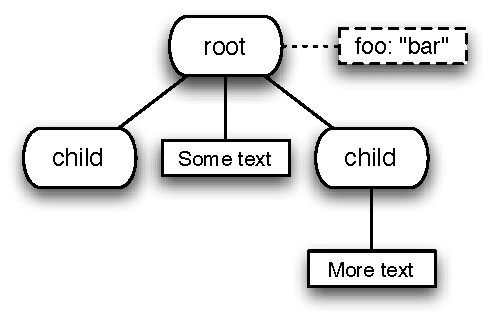
\includegraphics[width=5cm]{xml-example}
    \end{minipage}
  \end{tabular}
  \caption{A simple XML example}
  \label{fig:xml-example}
\end{figure}

\subsection{Namespaces}

XML  documents   may  contain  elements  and   attributes  from  different
vocabularies (i.e.~different document types). To resolve ambiguity between
the  involved   vocabularies,  the  W3C  recommends  the   use  of  unique
\emph{Namespaces}  that are  assigned  to each  element.   A document  may
contain a  \emph{default}-namespace to which  all elements belong  that do
not  have  a  special  namespace  assigned.   Within  a  single  document,
namespaces are given  a logical name. The logical  name itself is assigned
the unique  Namespace identifier (e.g.~an  \gls{glo:URI}). Some namespaces
and  common  ``names''   for  them  are  given  in   the  following  table
(Table~\ref{tab:namespaces}):

\medskip

\begin{table}[h]
  \centering
  \begin{tabular}{@{}ll@{}}\toprule
    logical name        & \multicolumn{1}{l}{namespace URI} \\ \midrule % header
    \texttt{xsd}        & \url{http://www.w3.org/2001/XMLSchema} \\
    \texttt{jsdl}       & \url{http://schemas.ggf.org/jsdl/2005/11/jsdl} \\
    \texttt{jsdl-posix} &  \url{http://schemas.ggf.org/jsdl/2005/11/jsdl-posix} \\
    \texttt{dsig}       & \url{http://www.w3.org/2000/09/xmldsig#} \\
    \texttt{bes}        & \url{http://schemas.ggf.org/bes/2006/08/bes-activity} \\
    \texttt{xbe}        & \url{http://xenbee.berlios.de/schemas/xbe/2007/01/xbe} \\
    \texttt{xsdl}       & \url{http://xenbee.berlios.de/schemas/xsdl/2007/01/xsdl} \\
    \bottomrule
  \end{tabular}
  \caption[XML Namespaces used in this work]{Important namespaces}
  \label{tab:namespaces}
\end{table}

Namespaces  are   specified  in  the  XML  using   the  special  attribute
\texttt{xmlns}.     An   attribute    of   an    element,    which   reads
\texttt{xmlns="www.example.com"}, sets the  default namespace to the given
URI, while  \texttt{xmlns:foo="www.example.com"} makes the  same namespace
known as the logical name  ``foo''. In another document the same namespace
could as well have been assigned the logical name ``bar''.

To specify  that a  given element  belongs to a  namespace other  than the
default namespace, the  element's name is prefixed by  the logical name of
the namespace,  e.g.~\texttt{foo:child} means, that  the ``child'' element
belongs to the namespace defined by ``foo''.

\subsection{Validation of XML documents}
\label{sec:xml-validation}

A  really nice  and very  useful  addition to  XML is  the possibility  to
\emph{validate}  an XML  document.  There  are two  mechanisms  to provide
validation,    the    \emph{Document    Type   Definition}    (DTD)    and
\emph{XML-Schema}.

\subsubsection{Document Type Definition}

A DTD defines for a particular  document what elements are allowed and how
their attributes look like. The  composition of elements to form container
(i.e.~parent)   elements  can   be   described  in   a  rudimentary   way.
Unfortunately, the  DTD uses  its own syntax,  that has nothing  in common
with  the syntax of  an XML  document. For  an author  of an  XML document
type\footnote{for example the configuration file format of an application}
that means in particular, that he has to learn two different syntaxes.

\subsubsection{XML-Schema Definition}

XML-Schema is  itself defined  using XML as  its description  language and
obsoletes the  DTD. It is much  more powerful, for instance,  an author is
able  to   restrict  the   actual  data  an   element  or   attribute  may
contain.  Let's for  instance  say, a  given  attribute can  only take  on
non-negative  integers.    To  reflect  this  constraint   in  the  schema
definition,  the   author  would  set   the  type  of  the   attribute  to
\texttt{xsd:nonNegativeInteger}.

There are many predefined data types, an author may use to create new data
type constraints.  An XML-Schema validator complains, if  a document, that
is  supposed to  conform  to  that schema,  contains  the just  introduced
attribute with a negative value, e.g.~$-1$.

\bigskip

The advantages of XML-Schema over a DTD are obvious.  When using DTDs, the
application  was  responsible to  check  the  validity  of each  used  XML
document  type  itself. That  means,  the  same  functionality had  to  be
implemented over and over again, i.e.~each time a new application wants to
make use of a given XML document type. While using XML-Schema definitions,
the author of  an XML document type defines  the validity constraints just
once and any application  may rely on that. To make that  clear, here is a
small  example:  Suppose there  is  a  definition  for an  element  called
``\texttt{entry-id}'',  which may  only take  on positive  integer values.
Since a DTD  does not support constraints on  data types, each application
must check  for itself if  the value matches  that type. Now  suppose, the
constraint  for  that  element is  changed,  so  that  the number  $0$  is
included, as  well ---  in each application,  the validation code  must be
modified to match the new constraint.

\section[Job Submission Description Language]
{Job Submission Description Language (\gls{glo:JSDL})}
\label{sec:fundamentals:jsdl}

\gls{glo:JSDL} is a very extensible XML-based description language for the
submission  of computational jobs.   With \gls{glo:JSDL}  you are  able to
describe  all requirements  that  a  computational job  may  need for  the
submission to  a remote resource  --- mainly the  \gls{glo:JSDL} addresses
grid resources but it is not limited the latter.

Nearly  every  element of  the  \gls{glo:JSDL}  specification may  contain
arbitrary  many  user-defined  elements  from  other  XML  specifications.
Therefore is the  JSDL fully adoptable to any  upcoming user requirements.
If  the  target  system,  for  instance, requires  a  previously  acquired
reservation ---  represented by an  identification number for  example ---
the  \gls{glo:JSDL} would include  an additional  element which  holds all
information regarding the reservation.  Such extension elements are purely
optional and  systems that are  unaware of a particular  extension element
may just neglect it.

The following section roughly describes the most important components that
are needed to form a useful submission description.

\subsection{``Hello World'' with the JSDL}

A    \gls{glo:JSDL}    document     does    always    start    with    the
\texttt{JobDefinition} element,  which is the top-level  element and holds
all required information about the job.

Let's assume a user wants to execute a small program on a remote resource.
The  program  will  indeed be  very  simple,  it  just prints  the  string
``\texttt{Hello World}'' to the  screen. The execution of this application
on the local computer of our user could be similar to:

\begin{minipage}{0.75\textwidth}
  \begin{lstlisting}[language=ksh]
    $ echo Hello World
    Hello World
    $
  \end{lstlisting}
\end{minipage}

This  excerpt  represents  the   execution  in  a  standard  UNIX  command
shell. Note that the \texttt{echo}  program does nothing more than writing
the parameters passed to it to its \texttt{stdout} stream. Now suppose the
user  desires  to execute  the  same program  on  a  remote resource,  the
\gls{glo:JSDL}  document, he  would  write, will  look  somewhat like  the
document shown in Listing~\ref{lst:jsdl-example}.

\bigskip

\begin{center}
  \begin{minipage}{.75\textwidth}
    \lstinputlisting[captionpos=b,backgroundcolor=\color{listingcolor},frame=lines,numbers=left,numberstyle=\tiny,caption={A
      small ``Hello World''-example written in
      \gls{glo:JSDL}},label={lst:jsdl-example},language=XML]{examples/jsdl-example.jsdl}
  \end{minipage}
\end{center}

Note, that  the shown \gls{glo:JSDL}  document describes exactly  the same
execution  the  user  had  previously  performed  locally.   The  executed
\texttt{echo} program  again writes  its arguments to  its \texttt{stdout}
stream.   Different from the  local execution  is in  this case,  that the
output will  be lost, since the  user did not  specify what is to  be done
with generated output. If the user was interested in the program's output,
he had to specify the redirection of  the output stream to some file and a
staging operation, that transfers the created file to some location he has
access to.

\subsection{Important elements}

A typical \gls{glo:JSDL} document consists  of the following parts --- job
identification,  application description,  resource descriptions  and data
staging elements. Only the first two of them have been used in the example
shown in Listing~\ref{lst:jsdl-example} to keep the example simple.

\subsubsection{Job identification}

The \texttt{JobIdentification}  element is used to  hold information about
the job, such as a descriptive  name, that is mostly interesting for human
beings.  Nonetheless it  may hold additional information that  could be of
interest to  applications processing the document ---  such as annotations
(e.g.~a  unique task  identification number  could  be stored  in such  an
annotation).

\subsubsection{Application}

With the \texttt{Application} element, a user describes the program itself
---  i.e.~the  real executable,  that  is going  to  be  used.  A  special
extension --- \texttt{POSIXApplication}, also defined in the specification
\cite{jsdl-spec}   ---   can  be   used   to   describe  executables   for
\gls{glo:POSIX}-compliant   operating  systems  \cite{posix}.    You  have
already      seen     the     usage      of     this      extension     in
Listing~\ref{lst:jsdl-example},  where it  had  been used  to specify  the
execution of the \texttt{echo} command line program.

\subsubsection{Resources}

This element can be used  to describe various resource requirements of the
application. Some of the many resource types one can use are listed below.

\begin{itemize}
\item the number of CPUs the job requires
\item the operating system required by the job
\item amount of virtual memory that must be available for the job
\item file-systems  and their expected  mount-points
\end{itemize}

All  specified file-systems  must  be  made available  for  the job  prior
execution. Every file-system specification  defines a unique name that can
be used to refer to that particular file-system in other elements, such as
staging operations.  Thereby the  user can define \emph{logical names} for
special directories within the execution environment of the task.
  
\subsubsection{Staging operations}

The   \texttt{DataStaging}    element   is   used    to   define   staging
operations.  These operations  can either  be  \emph{Stage-In} operations,
which  refer  to files  that  have to  be  transfered  into the  execution
environment  prior   the  execution  of  the   task,  or  \emph{Stage-Out}
operations, which refer  to transfers that have to be  made after the task
has been executed.

A user may  specify the \texttt{DataStaging} element as  often as he likes
to.   The most  relevant elements  within  a staging  instruction are  the
\texttt{Source}  and \texttt{Target}  elements, both  of them  can  hold a
\texttt{URI}  element  to  specify  a  generic  location.   The  mandatory
\texttt{FileName} element points to  an actual file within the file-system
hierarchy of the execution environment of the task. The actual location of
a file can be given relative  to a previously defined file-system, in this
case the \texttt{FilesystemName} element must be specified and is required
to contain the logical name of \texttt{FileSystem} resource.

\bigskip

As  you can  see,  the  \gls{glo:JSDL} is  a  really powerful  description
language and  it covers many,  if not all,  of the requirements  a typical
computational job  may have. And if it  does not cover a  special topic on
its own,  one is able  to extend the  elements of the  \gls{glo:JSDL} with
user-defined elements.

\section[Basic Execution Service]{The Basic Execution Service (BES)}
\label{sec:fundamentals:bes}

The \emph{Basic Execution Service} \cite{ogsa-bes} is a specification that
defines  a service (e.g.~a  web service)  which provides  functionality to
control \emph{Activities}.   A user is able  to submit an  activity to the
execution service and  can later on control and  monitor that activity ---
using web service calls, for instance.

Control  of  the  activity  is   basically  limited  to  a  request  which
\emph{terminates} the  activity. The monitoring of an  activity results in
returning the activity's current state.

The state  of an activity is  modeled using a finite  state automaton. The
specification of the \gls{glo:BES}  incorporates a rather simple, but very
extensible, state  machine for  activities. It comprises  a total  of just
five  states  an  activity  can  be  in  at  any  time:  \texttt{Pending},
\texttt{Running},       \texttt{Finished},       \texttt{Failed}       and
\texttt{Terminated}.

States of the \gls{glo:BES} are represented using a XML specification. The
element  which  represents the  current  state  of  an activity  is  named
\texttt{ActivityStatus} and belongs to  the \emph{bes} namespace as it has
been  defined  in Table~\ref{tab:namespaces},  the  state  itself is  then
specified using the \texttt{state} attribute:

\begin{lstlisting}[language=XML]
  <bes:ActivityStatus state="Running"/>
\end{lstlisting}

The     state     machine,     or     state-model,     is     shown     in
Figure~\ref{fig:bes-basic}. To  reflect the request for  termination of an
activity,  each state,  except the  final  states of  course, provides  an
outgoing transition to the \texttt{Terminated} state.

\begin{figure}[h]
  \centering
  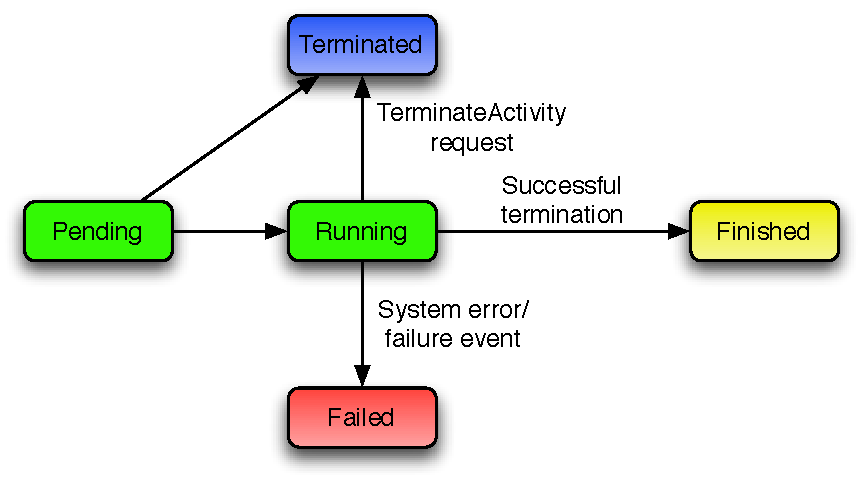
\includegraphics[scale=.6]{bes-basic-job-model}
  \caption[Basic BES Job-State-Model]{This is the job-state-model as it is
    defined in the BES specification \cite{ogsa-bes}}
  \label{fig:bes-basic}
\end{figure}

This very basic state-model represents everything a possible client of the
execution service needs  to know. An actual execution  service may require
to  use  additional  states.   It  can  define both  new  states  and  new
transitions,  as  long  as  it  conforms  to a  rather  simple  rule:  the
\textbf{visual behavior}, as it is experienced by some client, must not be
altered. A breakage of this rule would be the introduction of a transition
from  the \texttt{Running}  state  back into  the \texttt{Pending}  state.
Clearly, the visual behavior a  client experiences, has changed, since the
client  simply  does   not  expect  that  the  activity   is  suddenly  in
\texttt{Pending} again.

\subsection{Extending the state-model}

New states, for  instance, can be added by simply splitting  up one of the
``basic'' states.   Among these sub-states  any number of  new transitions
may be introduced.

Suppose the execution service provides  a way to suspend a given activity.
This  requires  not only  additional  user  requests  --- one  to  request
\emph{suspension} and  one to request  \emph{resumption} --- but  also two
new states. These states are modeled as sub-states of the \texttt{Running}
state, since an  activity may only be suspended  while it already running.
Thus,   the  \texttt{Running}   state   is  now   internally  split   into
\texttt{Executing} and  \texttt{Suspended}. The extended  state machine is
shown in Figure~\ref{fig:bes-suspend-model}

\begin{figure}[h]
  \centering
  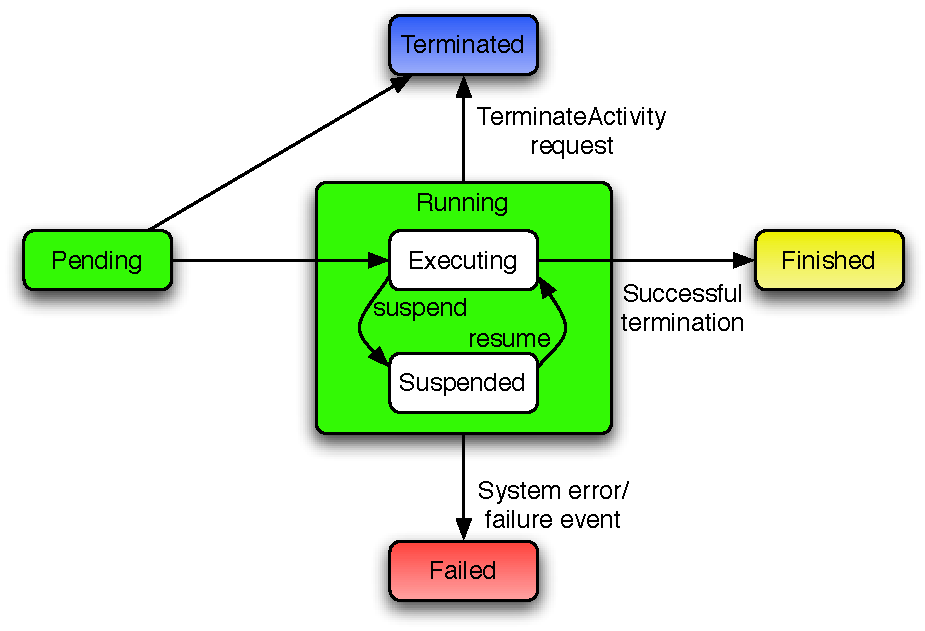
\includegraphics[scale=.6]{bes-suspend-job-model}
  \caption[Extended  BES Job-State-Model]{The  basic state-model  has been
    extended to support suspension.}
  \label{fig:bes-suspend-model}
\end{figure}

The nice  thing about the extensibility  of this state-model  is, that any
client  that  \emph{understands}  the  basic model,  will  understand  any
extended model  as well, that  is because the \emph{visual  behavior} does
not change  and therefore will never ``anything  unexpected'' happen. This
visual  behavior is  directly reflected  in the  XML specification  of the
current state.   Any additional  states are represented  by user-definable
elements attached to  the \texttt{ActivityStatus} element as sub-elements.
Let's  assume   the  extension  modeled   above  defines  its   own  state
representation  using its  own  namespace,  then the  current  state of  a
suspended activity could be written as:

\begin{lstlisting}[language=XML]
  <bes:ActivityStatus state="Running">
     <ext:Suspended/>
  </bes:ActivityStatus>
\end{lstlisting}

As you can see, the state  is still \texttt{Running}, but any client, that
is   aware    of   this   extension,   knows   how    to   interpret   the
\texttt{ext:Suspended} sub-element.

\section[Message Oriented Middleware]{Message Oriented Middleware (MOM)}
\label{sec:fundamentals:mom}

A  typical  way  of connecting  clients  with  some  server  is to  use  a
\gls{glo:TCP}-connection to the server for each client. This is especially
useful if a continuous connection to  the server has to be maintained. For
instance, web (i.e.~HTTP) and ftp (i.e.~FTP) servers are usually streaming
a lot of data to the clients.

Communication  in  distributed systems,  however,  can  take place  either
\emph{synchronously}, or  \emph{asynchronously}. The programming  model of
synchronous communication  is called \emph{Remote  Procedure Calls} (RPC),
widespread  implementations  of  this  model  are  CORBA,  RMI  and  DCOM.
Asynchronous   communication  follows   the  emerging   paradigm   of  the
\emph{event-based  communication  model}  \cite{MeCa:2005:Taxonomy}.   The
components that  comprise an application in a  potentially distributed and
heterogeneous   environment   are   asynchronously  interconnected   using
message-passing technologies.

\bigskip

\citet{dad-mom}  state, that  \emph{``Every  DAD (Distributed  Application
  Developer) needs a MOM (Message Oriented Middleware)''}.

Since the communication, which takes  place in the here proposed execution
environment and in  the later discussed Calana Grid  scheduler, is loosely
coupled  and message-oriented,  we  can abstract  from direct  connections
between each party to logical connections.

These logical  connections can be established using  a \gls{glo:MOM} based
on one or more \emph{message-queue servers} (\gls{glo:MQS}).

\gls{glo:MQS}   have  several  very   important  advantages   over  direct
connections between the clients and the server:

\begin{itemize}
\item All messages are  sent to \textbf{logical queues} (i.e.~end-points),
  that  means   that  the  physical  address  (e.g.~IP   address)  of  any
  participating  service  (be  it  the  server or  a  client)  may  change
  unnoticeable to the communication partner.
\item All connections are  \textbf{outbound}, which effectively means that
  the server may also reside behind a firewall or a \gls{glo:NAT}-gateway.
  This not only increases the security  of the server (in means of allowed
  inbound  connections),  but  also  targets the  problems  which  typical
  network-policies and  resulting network-layouts of  grid-environments or
  companies impose.
\item The  \gls{glo:MQS} need not  to be on  a single machine, but  can be
  distributed  over  many computers  to  implement \textbf{fail-over}  and
  \textbf{load-balancing}.
\item  Messages  are kept  in  a  \textbf{consistent  storage} within  the
  \gls{glo:MQS}, if they cannot be  delivered right now.  That may happen,
  if the communication partner is temporarily disconnected --- all pending
  messages will be delivered as soon as the end-point connects again.
\item    Multiple   \gls{glo:MQS}   can    be   configured    to   provide
  \textbf{forwarding and  routing} of  messages destined for  a particular
  queue --- that means independence from the actual network-topology.
\item A \gls{glo:MQS} can be configured to provide \textbf{authentication}
  and \textbf{authorization} to limit  access to (i.e.~send to and receive
  from) particular queues.
\item   Messages   sent   from   one   component   to   another   can   be
  \textbf{transformed}  while passing  the \gls{glo:MQS}.   That  means in
  particular,  that each  component may  send messages  in its  own native
  format and the \gls{glo:MQS}  intelligently transforms the messages into
  the native format of each receiver.
\end{itemize}



\begin{figure}[htbp]
  \centering
  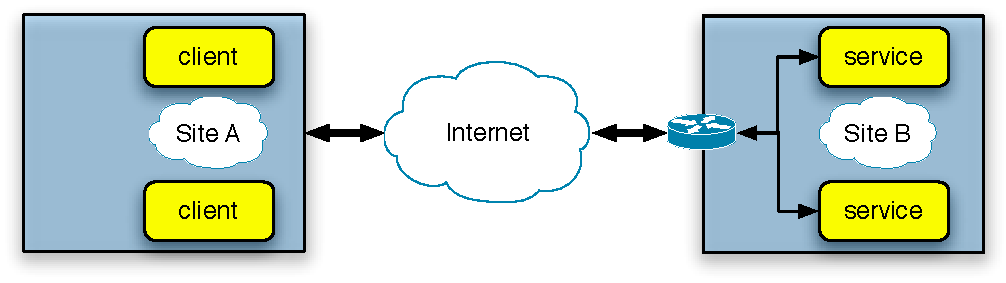
\includegraphics[scale=.5]{mqs-topology}
  \caption[Example MQS topology]{A simple message-oriented system which is
    using a \gls{glo:MQS}.}
  \label{fig:mqs-topology}
\end{figure}

As you can see in  Figure~\ref{fig:mqs-topology}, site B has some services
connected to  a \gls{glo:MQS}.  These services can  be reached  by clients
from site A through an internet connection. The steps involved in building
up this communication scheme are:
\begin{enumerate}
\item  Each service  connects to  the \gls{glo:MQS}  and \emph{subscribes}
  itself to a unique queue (e.g.~service.\emph{X}).
\item    Clients   subscribe    themselves   to    unique    queues,   too
  (e.g.~client.\emph{Y}).
\end{enumerate}

Now  that each  party is  subscribed to  its own  unique queue,  a two-way
communication is possible:
\begin{enumerate}
\item A client  that wants to communicate with one  of the services, sends
  its messages  to the unique queue  of that particular  service. The sent
  message  contains a  special \emph{reply-to}  field that  is set  to the
  unique queue of the client
\item Answers from  a service to a connected client are  sent to the queue
  specified in the reply-to field of received messages.
\end{enumerate}

\section{Secure Communication}
\label{sec:secure-communication}

The proposed system  will use message queues to  transfer messages between
clients and the server, that means  all messages that are sent can be read
by any person or system in between any two communication partners. 

A   typical  solution   to  make   the  transfer   secure  is   using  the
\emph{Transport Layer  Security} protocol --- or  \gls{glo:TLS} for short.
\gls{glo:TLS} makes sure that  traffic between two endpoints is transfered
securely --- i.e.~no eavesdropping, modification or message forgery.

The  \emph{Transport Layer  Security} protocol,  which is  discussed  in a
moment, and the afterwards examined \emph{Message Layer Security} protocol
are  both using cryptographic  certificates such  as \emph{\gls{glo:X509}}
certificates.

The  certificates  are  based  on  public/private  key  pairs,  whereas  a
certificate consists of a  pair's public-key combined with some additional
information, e.g.~the owner and issuer of the certificate, used algorithms
and  so  on.  Most  importantly  is the  fact,  that  certificates can  be
\emph{cryptographically    signed}     by    a    certificate    authority
(\gls{glo:CA}). The  next passage  will shortly describe  how certificates
can  be  used  in  a  \emph{Public Key  Infrastructure}  using  public-key
cryptography.

\subsection{Public-key cryptography}

Public-key  cryptography describes  a form  of cryptography  where  a user
holds  two  different  keys,  a  \emph{private  key}  and  a  \emph{public
  key}.  These two  keys are  mathematically  related to  each other,  but
nobody can practically derive the private key from the public key.

The public key can be made  publicly available without any risk, while the
private key must  be kept very secret. A widely used  algorithm is the RSA
algorithm named  after its  creators \citet*{rivest77method}. It  has been
the first algorithm, that  was suitable for both encryption/decryption and
signing.  For more background information on public-key cryptosystems, you
are encouraged to read \cite{rivest77method,diffie76new}.

The RSA algorithm relies on the fact, that the factorization of reasonably
large numbers is  computationally very hard and no  efficient algorithm is
publicly known.  Especially  hard to factor are numbers  whose factors are
two randomly-chosen prime numbers of sufficient length.

In the following  I am going to describe  how the keys are set  up and how
they are used to encrypt/decrypt or to sign/validate a clear text message.

According  to  \cite{rivest77method},  places  each  user  his  encryption
procedure $E$  in a publicly accessible file  (e.g.~database).  Using this
public file, any  other user is able to  retrieve the encryption procedure
of   some  other   user  (i.e.~the   one  he   wants  to   send  encrypted
messages). Each user keeps his decryption procedure $D$ secret.

The mentioned procedures $D$ and $E$ have the following properties:
\begin{enumerate}
\renewcommand{\theenumi}{\alph{enumi}}
\renewcommand{\labelenumi}{(\theenumi)}

\item Deciphering  the enciphered form of  a message $M$  yields $M$. That
  is,
  \begin{equation}
    \label{eq:1}
    D(E(M)) = M.
  \end{equation}
  \label{pubkey-cryptosystem-prop-1}
\item Both $D$ and $E$ are easy to compute.
  \label{pubkey-cryptosystem-prop-2}
\item The user does not reveal an  easy way to compute $D$ if he makes $E$
  publicly available.
  \label{pubkey-cryptosystem-prop-3}
\item  The enciphering  of a  previously ciphered  message $M$  results in
  $M$. That is,
  \begin{equation}
    \label{eq:1}
    E(D(M)) = M.
  \end{equation}
  \label{pubkey-cryptosystem-prop-4}
\end{enumerate}

A                  function                 $E$                 satisfying
(\ref{pubkey-cryptosystem-prop-1})--(\ref{pubkey-cryptosystem-prop-3})   is
said  to  be  a  \emph{``trap-door  one-way function''}  and  if  it  also
satisfies  (\ref{pubkey-cryptosystem-prop-4})  it  is a  \emph{``trap-door
  one-way permutation''} \cite{rivest77method,diffie76new}.

\subsubsection{Key setup}

The \emph{encryption  key} consists  of a pair  of positive  integers $(e,
n)$,  where $e$  is the  \emph{encryption exponent}  and $n$  is  used for
modulo  operations.  The \emph{decryption  key}  is  also  a pair  of  two
integers, where only the exponent differs, thus $(d, n)$ is the decryption
key and $d$  represents the \emph{decryption exponent}. $(e,  n)$ are made
publicly available.

\citet*{rivest77method} suggest the  following approach for the generation
of $(e, n)$ and  $(d, n)$. The fist step is to  compute $n$ as the product
of two very large, ``random'' primes $p$ and $q$:
\begin{equation*}
n = p \cdot q.
\end{equation*}

Although you  publish $n$, nobody is  able to compute the  factors $p$ and
$q$ in  reasonably time due to  the enormous difficulty  of factoring $n$.
In \cite{rivest77method}  it is assumed,  that the computation of  $p$ and
$q$ from a given $n$ takes $1.5 \times 10^{29}$ operations, given that $n$
has a length  of $300$ digits. If one operation  took one microsecond, the
whole computation takes $4.9 \times 10^{15}$ years.

The  next step  is to  choose  $d$, therefore  one picks  a large,  random
integer that is \emph{co-prime}\footnote{two integers $a$ and $b$ are said
  to be co-prime  if they do not  have a common factor other  than $1$ and
  $-1$, i.e.~their greatest common divisor  (gcd) is $1$.} to $(p-1) \cdot
(q-1)$.\footnote{the term $(p-1)\cdot(q-1)$ is the result of \emph{Euler's
    Phi} or  \emph{Euler's totient function}  ($\phi$) applied to  $n$} In
other words, $d$ has to satisfy:
\begin{equation*}
  gcd(d, (p-1) \cdot (q-1)) = 1.
\end{equation*}

Finally,  the integer $e$  is computed  from $p$,  $q$ and  $d$ to  be the
\emph{multiplicative inverse} of $d$, modulo $\phi(n)$:
\begin{equation*}
  e \cdot d \equiv 1\ \ (mod\ (p-1) \cdot (q-1))
\end{equation*}

\subsubsection{Encryption and Decryption}

If  two  persons,  Alice  and   Bob,  want  to  send  each  other  private
(i.e.~encrypted)  messages,  they   both  retrieve  the  other's  publicly
available encryption  key first ---  Bob retrieves $(e_a, n_a)$  and Alice
retrieves $(e_b, n_b)$.

Let's say  Alice wants to send a  private message to Bob.   To encrypt the
message, she has to  represent it as an integer between $0$  and $n_b - 1$
(long  messages can  be broken  into smaller  blocks, so  that  each block
fulfills the requirement). Alice then  encrypts the message $M$ by raising
it to the $e_b$th power modulo $n_b$, the result is the cyphertext $C$:
\begin{equation*}
  C \equiv E(M) \equiv M^{e_b}\ \ (mod\ \ n_b).
\end{equation*}

On reception  of the cyphertext  $C$, Bob raises  it to the  $d_b$th power
modulo $n_b$. He  is the only person, who knows $d_b$  and therefore he is
solely able to decrypt $C$:
\begin{equation*}
  M \equiv D(C) \equiv C^{d_b}\ \ (mod\ \ n_b).
\end{equation*}

\subsubsection{Signing and Validating}

Electronic  signatures, e.g.~in electronic  mail systems,  especially when
used in  business transactions, must  provide provability to  the receiver
that  the message  originated from  the sender.   This is  more  than just
provide  mere \emph{authentication},  where the  recipient of  a digitally
signed message can  verify that the message came  from the sender. Digital
signatures must be  able to be used to convince  a ``judge'', that neither
the recipient did  forge the message, nor the sender  can deny sending the
message.

That means,  an electronic signature must  be \emph{message}-dependent, as
well as  \emph{signer}-dependent. If the  signature did not depend  on the
message itself, a dishonorable recipient  could just change the message or
attach the signature to a  completely different message before showing the
message/signature pair  to a judge. If  the signature would  not depend on
the \emph{signer}, obviously anybody could have signed the message.

\medskip

If   Bob  want  to   send  Alice   a  signed   message,  he   applies  his
\emph{decryption}  function $D_b$  to the  clear text  message  $M$, which
results in the signature $S$:

\begin{equation*}
  S = D_b(M).
\end{equation*}

To   perform  this,   the  cryptosystem   has  to   be   implemented  with
\emph{trap-door         one-way        permutations},        i.e.~property
(\ref{pubkey-cryptosystem-prop-4}) must hold.

This signature  can now  be encrypted using  Alice's public key  to ensure
privacy, there  is no need to  send the message along  with the signature,
since it can  be computed from it. On reception,  Alice first decrypts the
message which  results in the  plain signature $S$ again.   Applying Bob's
\emph{encryption} function to the  received signature (Alice knows who the
presumed sender  of the  message is) makes  perfect sense due  to property
(\ref{pubkey-cryptosystem-prop-4}):

\begin{equation*}
  M = E_b(S)
\end{equation*}

Bob cannot  later on deny that he  sent the message, since  nobody but him
could  have generated  the signature  $S$.  Alice  is able  to  convince a
``judge'', that  Bob did send the  message, since $E_b(S) =  M$. But Alice
cannot modify  $M$ or  provide a different  message $M'$ because  then she
would also need to compute $S' = D_b(M')$ as well.

\subsection[Public Key Infrastructure]{Public Key Infrastructure (PKI)}

A  \emph{Public Key  Infrastructure} provides  the authentication  of user
identities using certificates.  The main  aspect is that there are special
\textbf{trusted    third     parties}    (\emph{Certificate    Authority},
\gls{glo:CA}), that are permitted  to \textbf{sign} other certificates. If
a  user\footnote{or some  server, etc.}   wants to  prove his  identity to
another entity,  his certificate is  validated by that entity  against the
CA's certificate, if it is valid, the prove has been successful.

The \gls{glo:CA} is responsible for checking that the public-key contained
in  the certificate  actually belongs  to the  requesting user,  server or
other  entity denoted  in the  certificate. This  checking process  is for
example done by  verifying the credentials of a user  (e.g.~with help of a
photo identification or something similar).

Any third-party that trusts a given CA will transparently trust any entity
that offers a certificate signed by that particular CA.

\begin{figure}[h]
  \centering
  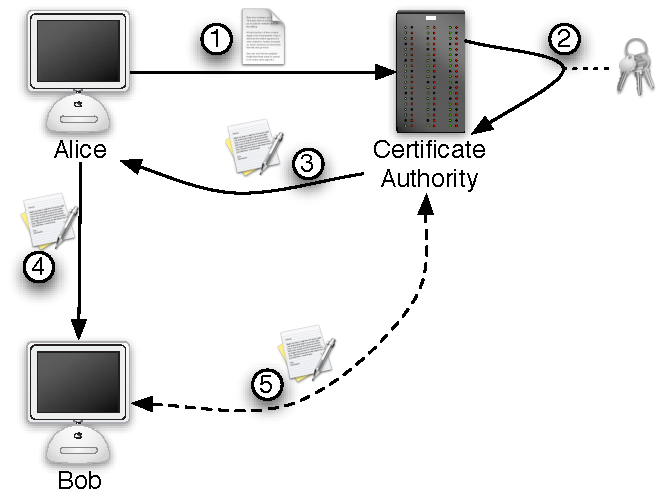
\includegraphics[scale=.75]{pki}
  \caption[Public  Key Infrastructure]{Alice  proofs her  identity  to Bob
    using a certificate  that is signed by a CA that  both, Alice and Bob,
    trust.}
  \label{fig:pki}
\end{figure}

Validation is performed by verifying  that the certificate itself has been
signed  by a  trusted authority  --- the  actual validation  process  is a
little   bit  more  complex,   since  it   involves  checking   against  a
\emph{Revocation List} and  a ``best before'' date (i.e.~life  time of the
certificate), too.

The  signing  process  uses  the  authority's private  key  to  compute  a
cryptographic signature. This private-key must of course be kept in a very
secure  location  (e.g.~on a  physically  from  the Internet  disconnected
computer) ---  if it would fall into  the wrong hands, the  whole chain of
trust is compromised.

An  example verification  process  is shown  in Figure~\ref{fig:pki},  the
steps can be described as follows:
\begin{enumerate}
\item \emph{Alice} request the signing of her certificate by a CA and thus
  sends a certificate request to the CA containing her public-key.
\item The CA in turn verifies Alice's credentials and eventually signs the
  certificate with its private key.
\item The signed certificate is sent back to \emph{Alice} for her later use.
\item Now,  \emph{Alice} wants to prove  her identity to a  friend of her,
  \emph{Bob},   therefore   \emph{Alice}    sends   her   certificate   to
  \emph{Bob}.  The   proof  may  be   necessary  to  establish   a  secure
  communication over an insecure channel, e.g.~the Internet.
\item \emph{Bob}  verifies the received certificate against  the very same
  CA by  which \emph{Alice} had her certificate  signed.  Since \emph{Bob}
  trusts the  CA and the received  certificate states, that  it belongs to
  his  friend \emph{Alice},  he  can be  assured,  that he  is talking  to
  \emph{Alice}.
\end{enumerate}

\bigskip

Both  of  the following  protocols  can make  use  of  a \gls{glo:PKI}  to
authenticate communication partners.

\subsection[Transport Layer Security]{Transport Layer Security (TLS)}

The \gls{glo:TLS}  protocol is often  offered by web- or  email-servers to
make  the  communication   with  a  client  (such  as   a  browser  or  an
email-client) secure.

On-line   banking,   for   instance,   typically   requires   a   Personal
Identification Number  (PIN) to make sure  that it is actually  you who is
trying to access your accounts.  Using unencrypted transfer of the PIN and
other data would mean, that any  system, which is in between your computer
and the  one of your  bank, is  able to read  your PIN and  probably other
information about you. It is also possible that a \emph{man-in-the-middle}
spoofs or modifies  transactions to withdraw money from  your account. Two
things are  very important in  this case: The  first and most  obvious is,
that the information you and  your bank exchange are encrypted. The second
requirement is,  that you  are able  to verify that  the receiver  of your
messages is actually a computer belonging  to your bank and not to someone
else.

\gls{glo:TLS} uses  certificates on the  server-side, so that  clients can
validate  that  they  are  actually  communicating with  the  server  they
intended to  communicate with.  In  the case of  a bank or  any well-known
service  provider   in  the  Internet,  the  certificates   in  place  are
cryptographically  signed by a  \emph{trusted} authority.   A certificate,
that is signed by such an authority you trust, is automatically assumed to
actually belong to the server where the certificate came from.

\bigskip

Unfortunately, \gls{glo:TLS}  cannot be used in a  message-queue system to
secure the traffic  between clients and servers. That  is because there is
no direct connection between client and server --- both are just connected
to their message-queue server. \gls{glo:TLS} can in this case only be used
to secure  the communication between  any end-point and  the message-queue
server it  is connected to.

After transmitting a message over a with \gls{glo:TLS} secured connection,
the  message is  stored in  clear text  on the  message-queue  server. The
message   will  then   again  be   transmitted  securely   to   the  final
destination. But  any person  or system with  access to  the message-queue
server can read, modify or even spoof transmitted messages --- without the
knowledge of either sender or receiver.

To  secure  the  logical   message-based  communication  between  any  two
end-points, a  different kind of security  layer has to be  used here: the
\emph{Message Layer Security} --- or \gls{glo:MLS} for short.

\subsection[Message Layer Security]{Message Layer Security (MLS)}

As the name of this protocol  may already suggest, the security focuses on
the transmitted messages not on  the transportation of the messages.  That
means, the transport layer over which  messages are sent is not altered or
secured in any way  --- it can be as insecure as  before.  But even though
the messages are transmitted over a potentially insecure channel, they are
still protected against eavesdropping, tampering and spoofing.

\gls{glo:MLS} too makes use  of certificates to provide authentication and
encryption. To  establish a  secure communication between  a client  and a
server,  the  client  needs  to  \emph{know}  (i.e.~have  access  to)  the
certificate  of the server.   Since encryption  with a  public/private key
algorithm   is    rather   slow,    in   most   cases    a   \emph{session
  key}\footnote{typically  random data}  will be  negotiated  first.  This
session  key is  then used  to perform  \emph{symmetric} ciphering  of the
messages, which is a lot faster.

\bigskip

The \gls{glo:XenBEE}  must make use  of \gls{glo:MLS} to  provide security
for  its users.   Additionally, as  it is  common  among Grid-middlewares,
\gls{glo:X509}  certificates  are   used  to  authenticate  and  authorize
users. The  server is going  to use a  user's certificate to  validate his
identity and  possibly to send messages  the user --- thus  both sides may
initiate a secure communication.

\section{Calana}
\label{sec:calana}

\emph{Calana} is  a new  Grid-scheduler approach proposed  by M.~Dalheimer
\cite{dalheimer05agentbased}.  The  scheduler uses \emph{agents}  that are
responsible for  a single  resource and at  least one  \emph{broker}.  The
broker initiates an \emph{auction} among  the connected agents to assign a
task to some resource.

\begin{figure}[htbp]
  \centering
  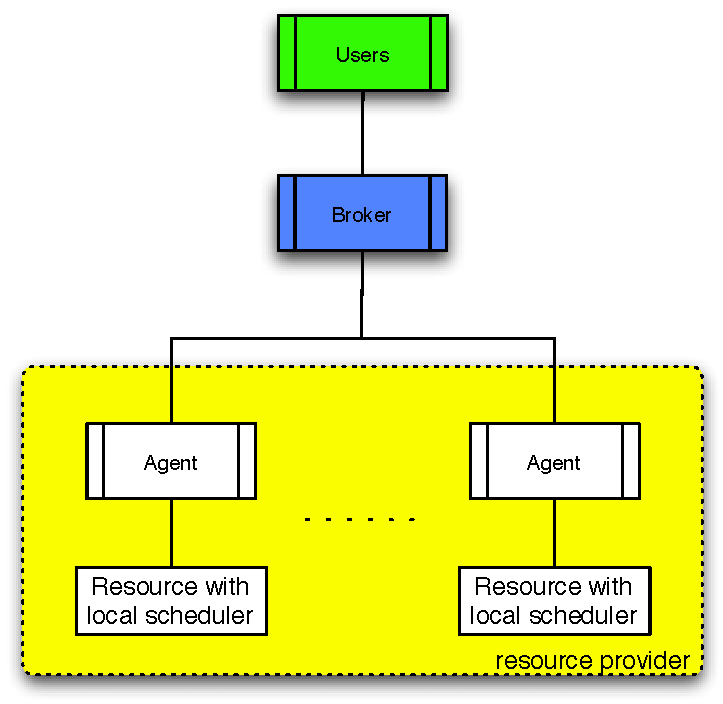
\includegraphics[scale=0.5]{calana-architecture}
  \caption{Architecture of Calana}
  \label{fig:calana-architecture}
\end{figure}

An  abstract   view  over   the  architecture  of   Calana  is   shown  in
Figure~\ref{fig:calana-architecture}.   For a  detailed discussion  of the
Calana-protocol  that  is used  to  perform an  auction,  have  a look  at
\cite{dalheimer06calanaprotocol,petry06}, but  the  main steps  involved
are:
\begin{enumerate}
\item When a user submits a job to the Calana-broker, the broker will open
  up an auction and try to \emph{book} a resource for the task.
\item    For   each   task    an   auction    is   created    by   sending
  \texttt{BookingReq}-messages to the connected agents.
\item The agents will make  one or more \emph{reservations} on their local
  scheduler  and  answer with  a  \texttt{AuctionBid}.   Bids contain  for
  example  the  cost  of   using  the  resource  and  various  reservation
  parameters  such  as  the   earliest  start-time  and  duration  of  the
  reservation.
\item To make a decision, the  broker judges all received bids and chooses
  the     best     one      according     to     some     preference-model
  \cite{dalheimer05agentbased, petry06}.
\item If  the user  accepts the decision,  the broker  \emph{confirms} the
  reservation.
\end{enumerate}

%%% Local Variables: 
%%% mode: latex
%%% TeX-master: "main.tex"
%%% End: 
